% THIS IS SIGPROC-SP.TEX - VERSION 3.1
\documentclass{llncs}

% Additional packages
\usepackage{graphicx}
\usepackage{color}
\usepackage{url}
\usepackage{algorithm}
\usepackage[noend]{algpseudocode}
\usepackage{amsmath}
%\usepackage{amsthm}
\usepackage{amsfonts}
\usepackage{amssymb}
\usepackage{booktabs}
\usepackage{multirow}
\usepackage{ifpdf}
% Custom commands
\usepackage{custom_commands}

%\newcommand{\prg}[1]{\paragraph{#1}}
\newcommand{\prg}[1]{\textbf{#1}.}

\renewcommand{\note}[1]{{\color{red}{#1}\par}}
\renewcommand{\note}[1]{}

\newcommand{\Siren}{\textsc{Siren}}
\newcommand{\ReReMi}{\textsc{ReReMi}}

\def\verExample{1}
\def\verE{0}

\begin{document}

\title{A Case of Visual and Interactive Data Analysis: Geospatial Redescription Mining\thanks{This is a pre-print version of the original article presented at the ECML PKDD 2012 Workshop on
Instant Interactive Data Mining}}

%\numberofauthors{2} 
\author{
Esther Galbrun\inst{1}
\and
Pauli Miettinen\inst{2}
}

\institute{
  Helsinki Institute for Information Technology,\\
  Department of Computer Science, \\
  University of Helsinki, Finland,\\
  \email{galbrun@cs.helsinki.fi}
\and
  Max Planck Institute for Informatics, \\
  Saarbr{\"u}cken, Germany,\\
  \email{pmiettin@mpi-inf.mpg.de}
}
 
\maketitle
\begin{abstract}
  We present a method for visual and interactive geospatial
  redescription mining. The goal of geospatial redescription mining is
  to characterize geospatial areas using two different descriptions,
  such as their bioclimatic features and fauna. Indeed, one
  application of geospatial redescription mining is finding
  bioclimatic niches, i.e. explaining the distribution of species
  using their bioclimatic envelope.

  Allowing users to find the geospatial redescriptions in an
  interactive way, and to see the results in clear visualizations, is
  fundamental for the applicability of the method. We present several
  goals we think a good interactive and visual redescription mining
  method should fulfil, and we explain how our proposed method
  achieves (most of) them. Finally, we also discuss some open problems
  in interactive redescription mining.
\end{abstract}

\section{Introduction}
\note{TODO: start visual and interactive data mining more generally?}

Finding multiple ways to characterize the same entities is a problem
that appears in many areas of science.  In medical sciences, one might
want to find a subset of patients sharing similar symptoms and similar
genes. Describing geographical regions in terms of both their
bioclimatic conditions and the fauna that inhabits them is another
example.  A simple example of a redescription in this setting could
state that areas where Moose live are areas where February's maximum
temperature is between $-10$ and $0$ degrees Celsius and July's
maximum temperature between $12$ and $25$ degrees Celsius.
%This is actually the redescription shown in the foreground panel of
%Figure~\ref{fig:both_panels}.
\note{maybe we do want to have some screenshot already here, maybe
  not...}
\note{I'd even say yes we want.}

The results of redescription mining, the redescriptions, can be
approached from two points of view. On one hand, by considering the
variables and conditions appearing in the queries, which provide
valuable information in themselves; on the other hand, by studying the
support set of the redescriptions, i.e.\ the subset of entities where
both queries of a redescription hold. 
 
\note{This explanation is unclear about split between visualization
  and interactivity and dependance between two.}
\note{But does it matter? I'm not religious about splitting the two --
I don't think it works, in fact -- but I think that presenting the
goals with split is easier than in a merry mess of all of them.}
To analyse the
redescriptions, the ability to visualize the support sets is very
helpful. With geospatial data, the visualization is rather simple:
plot the support sets in a map. But just plotting the results on a map
is not enough: the user must also be able to interact with the
program. This interaction can be conceptually divided in two
sub-phases: interacting with the data mining algorithm and interacting
with the result visualization. A third level of interaction happens
between these two conceptual phases: the user moves back-and-forth
between issuing commands to find new results and examining the
already-found results. We argue that a good interactive data mining
tool should facilitate all three types of interaction. In this paper
we discuss about ways to facilitate this interaction in the process of
mining redescriptions. We then present a pair of algorithms, \ReReMi\
and \Siren, and explain how they implement interactivity and
visualization for redescription mining. Lastly, we discuss some
possible pitfalls associated with interactive, visual redescription
mining. But first, we formally define the redescription mining
problem.

%%% Local Variables: 
%%% mode: latex
%%% TeX-master: "siren_iid"
%%% End: 

\section{Redescription Mining}
\label{sec:redescription-mining}

\note{It might not hurt to have one more example in this chapter, if
  space permits.}
Redescription mining aims at simultaneously finding multiple
descriptions of a subset of entities which is not previously
specified.  This is in contrast with other methods like Emerging
Patterns Mining (EPM), Contrast Set Mining (CSM) and Subgroup
Discovery (SD) (see \cite{kralj09supervised} for a unifying survey) or
general classification methods, where target subsets of entities are
specified via labels.  Currently, redescription mining is a purely
descriptive approach, its predictive power remains to be explored.
Since its introduction in~\cite{ramakrishnan04turning} various
algorithms have been proposed for Boolean redescription mining, based
on approaches including decision
trees~\cite{ramakrishnan04turning,kumar07redescription},
co-clusters~\cite{parida05redescription}, and frequent
itemsets~\cite{gallo08finding}. In~\cite{galbrun11black}, we extended
redescription mining to categorical and numerical variables.

More formally, we consider data that contains entities $E$ with two sets
of characterizing variables, e.g.\ the fauna and the bioclimatic
conditions. 
Boolean variables can be interpreted as a truth value
assignment in a natural way.  For categorical and real-valued
variables, truth value assignments are induced by relations denoted using Iverson bracket $[v=c]$
and $[a \leq v \leq b]$, respectively, where $c$ is some category and
$[a, b]$ an interval.  These truth assignments and their negations
constitute \emph{literals} which can be combined using the Boolean
operators $\land$ (and) and $\lor$ (or) to form \emph{queries}.
The support of a query $q$ is the subset of entities for which
the query holds true, that is 
$\supp(q) = \{e\in E : q\text{ is true for } e\}$.
We refer to the two sets of variables informally as left and right
hand side data, and the queries over them as left and
right hand side queries, denoted as  $q_\iLHS$ and  $q_\iRHS$, respectively.
Then, a redescription is simply a pair of queries over variables from the
two sets, $R=(q_\iLHS,q_\iRHS)$.    
Its \emph{accuracy} is 
measured using the \emph{Jaccard coefficient} 
\[
\jacc(R)= \jacc(q_\iLHS,q_\iRHS) = \frac{\abs{\supp(q_\iLHS,q_\iRHS)}}%
{\abs{\supp(q_\iLHS)\cup\supp(q_\iRHS)}}.
\]
We compute a \pValue{} that represents the probability that two random
queries with marginal probabilities (i.e.\ the fraction of entities
supporting them) equal to those of $q_\iLHS$ and $q_\iRHS$ have an
intersection equal to or larger than $\abs{\supp(q_\iLHS,
  q_\iRHS)}$. This probability uses the binomial distribution and is given by \[
\text{pvalM}(q_\iLHS, q_\iRHS) = \sum_{s=\abs{\supp(q_\iLHS, q_\iRHS)}}^{\abs{E}} {\abs{E} \choose s} (p_R)^s (1- p_R)^{\abs{E} - s},\]
where $p_R = \abs{\supp(q_\iLHS)}\abs{\supp(q_\iRHS)}/\abs{E}^2.$
The higher the \pValue, the more likely it is to observe such a
support for independent queries, and the less significant the query.

The task consists in finding significant accurate redescriptions, in other words, pairs of
queries, one query for both sets of variables, such that both queries
describe almost the same set of entities.

When the data is geospatial, that is, the entities are connected to
geographical locations, the task is called \emph{geospatial redescription mining}.
 A meaningful geospatial redescription should define
coherent areas using expressive queries.

\emph{Niche-finding} is a particular instance of geospatial redescription
mining ---and a task of great importance for biologists.  The
bioclimatic constraints that must be met for a certain species to
survive constitute that species' bioclimatic envelope, or
niche~\cite{grinnell17niche}.  Finding such envelopes can help, e.g.\
to predict the results of global warming~\cite{pearson03predicting}.
A number of methods, involving regression, neural networks, and
genetic algorithms (see~\cite{soberon05interpretation}) have been
developed over the past ten years to model the bioclimatic envelope,
\textsc{Maxent}~\cite{phillips2006maximum} and \textsc{BIOMOD}~\cite{thuiller09biomod}, being good examples of a
modelling tools used in this domain, the former providing a graphical user interface while the latter is a text-based tool.  But to the best of our knowledge,
none of these methods allows automatically finding both the set of
species and their envelope.

%%% Local Variables: 
%%% mode: latex
%%% TeX-master: "siren_iid"
%%% End: 


\section{Goals for Interactive and Visual Redescription Mining}
\label{sec:goals-inter-visu}

In this section we discuss our goals for an interactive and visual
redescription mining tool. Some of these goals are general to any
interactive and visual data mining tool (and we spend less time on
discussing why they are desirable), some are specific to
redescription mining. We divide the discussion between interaction and
visualization, though we emphasize that these goals are not independent.

\note{By no means to do I mean that we should follow some orthodox
  dichtonomy between visualization and interaction. They are
  interlinked, and that's fine. My goal is to ease the presentation by
  giving the user some high-level structure. If something is both
  visualization and interaction, we can mention it in both, putting
  emphasizis on where it belongs more.}

\subsection{Visualization of Results}
\label{sec:goals-visualization}
As a basis for our discussion, we use the taxonomy of interactions for
visual analytics proposed by Heer and
Shneiderman~\cite{Heer:2012:IDV:2133806.2133821}. The bold-face terms
correspond to their taxonomy.

\note{Filter \& sort refers to filtering and sorting what's
  visualized, right. So, yes, actions to lists of redescriptions are
  there, but also (a feature we sort-of have) selecting the geospatial
  area where we see the dots (zooming in/out) is filtering. These
  things don't need all to be grand and sexy, but they have to be.}
\note{I don't quite agree with zooming as filtering, and zooming is
  mentioned later anyways} The most fundamental goal when designing a
tool for visual data analysis is, of course, to have a good
\textbf{visualization}. With geospatial redescriptions, a map is the
most natural option. Thus our tool should be able to plot the
redescriptions on a map. But in order to effectively select the
content of the visualizations, the user needs means to \textbf{filter}
and \textbf{sort} the results mined. In the case of redescription
mining, the user should be able to sort the returned redescriptions
based on different criteria, such as accuracy, support size,
statistical significance, or query length (i.e.\ number of literals).
To some extent, filtering can be regarded as sorting with a cut-off
value. Hence, sorting should naturally use the same criteria and
similar results display as sorting. Additional criteria might affect
sorting, including the described geographical area and redundancy.

During the analysis, the user should be allowed to \textbf{derive} new
data. That is, new variables obtained by aggregating existing
variables might better capture the studied phenomenon. Hence, their
introduction during the mining process would support the
analysis. While modifying the way the information is represented,
deriving new variables is also a mean to interact with the mining
process.

\note{One can select a redescription to visualize, select an area of
  interest, a particular entity.  We do not have different levels of
  details, so, there is not much to navigating...}  \note{In addition,
  the user should be able to select a geographical area and get info
  on the data on that area. Remember the pop-up window I mentioned?
  Further levels of detail could come from whether she sees the info
  for just the variables involved in the queries, or for all
  variables.}  In order to manipulate the views, the user needs to be
able to \textbf{select} the data he wants to visualize. In the present
case, he can primarily choose a redescription to plot. Then, he can
edit the queries, modifying literals and altering the bounds of real-valued variables.  The user might need to \textbf{navigate} inside the
view, typically looking first at the redescription over the whole
area, before zooming and panning to see more details. On a high level,
the user might only be able to see whether either query hold on a
region. Focusing on particular area, he might obtain more detailed
information about the actual state of the variables and what makes a
query hold or not in a particular location, for instance by clicking
or hovering over a dot in the map. Several views and the data might
need to be \textbf{coordinated}.  Modifications made to a
redescription should be reflected immediately on the map(s). In
addition, it could be useful to allow the user to bind maps together,
so that panning and zooming are applied to all maps simultaneously. In
that way, detailed comparison of the support of different
redescriptions would be facilitated.  Maps can be opened in detachable
tabs, to be inspected side by side or sequentially and be
\textbf{organized} using the system's or a dedicated windows tiling.

For any interactive tool, undo and redo are minimal functionalities to
allow reverting actions, making interaction safe and comfortable.  The
user should be able to save the current status of the analysis
process, i.e. all current redescriptions, opened lists and maps to
punctuate the process. \textbf{Recording} the interaction history and
turning it into editable and parameterizable macros provides a mean to
repeat a sequence of actions and automate repetitive tasks.  The tool
should support \textbf{annotation} in order to keep track of the
thought path during the analysis.  For example, this could be achieved
by generating annotable screen shots of the current window of
interest, and by adding comments to the interaction history and
macros.  Organizing the history and macros into blocks would help
clarifying the logical structure of the analysis.  Furthermore, with
the ability to link to objects in the current environment such as
redescriptions, groups of entities or literals, they could be
explicitly related to each other.  Data analysis is often a
collaborative effort, involving several users. Then, \textbf{sharing}
information becomes crucial.  Easy export and import of redescriptions
lists, maps and macros, possibly with comments and annotations is a
very important feature towards that aim.  Finally, giving clear names
to the actions and providing feedback on their application helps
\textbf{guiding} users along the analysis process. Example macros with
detailed explanations, to be replayed step-by-step, represent a good
mean to introduce new users to the tool.  These latter goals pertain
automating interactions, attaching a meaning to sequences of
interactions, allowing segmented interactivity, e.g. when different
users collaborate, using the tool in turn. Hence they are also closely
tied to the interaction with the mining process, to which we now turn.

\subsection{Interaction with the Mining Process}
\label{sec:goals-interaction}

A desirable behavior for an interactive program is the production of
meaningful results at \goal{any time}.  In other words, if the mining
process is stopped, it can nevertheless return results which are
valid, albeit possibly partial.  This is related to the possibility to
obtain preliminary results while the mining is still underway.  Such a
feature contributes to the ability of the program to respond quickly
to instructions from the users.  It is also possible to first run the
algorithm allowing only short queries, say, at most a couple of
literals on either side and let the user choose the ones that seems
promising and should be further extended. Low latency or even
\goal{instantaneity} is a core quality of an interactive tool and is
important catch and keep the user's attention. At least, the tool
should provide instant feedback about what is happening.

The automation level of the whole mining process could be adaptative.
From fully manual, where the users writes down redescriptions and the
tools simply evaluates them, to fully automated where the program
mines the list of best redescriptions using static predefined
constraints, it could also be partially automated, with the tool
suggesting best extensions at each step and asking for approval from
the user.

Consider extending an existing redescription with a real-valued
literal. Instead of a map plot based on their geographical location, a
figure where the areas are represented as colored dots plotted along
the $x$-axis depending on the value taken by the chosen variable would be
useful for determining the optimal interval for that variable. Indeed,
the user could observe which values occur in locations that belong to
different parts of the current redescription. Then, he could fix the
bounds in consequence, for example using sliders.  The tool could even
indicate which are the best bounds but also update the best
corresponding upper bound when the user moves the lower bound, and
vice versa. This is a prime example of instant interaction with the
mining process through apt visualization.  \note{We might need an
  illustration for that one...?}

Proper interactivity with the program also requires allowing the user
to specify constraints for the search. Possible constraints include
specifying variables or geographical areas that should be excluded
from the redescriptions or modifying the minimum acceptable accuracy.
For such constraints that constitute filtering criteria, there can be
three different degrees of integration with the algorithm, that is of
how far they are pushed into the mining process instead of applied a
posteriori.  The degree zero of integration happens when the user
manually filters the raw output. Instead, the program can
automatically filter its results before reporting. The highest degree
of integration implies incorporating such filtering criteria during
the search to avoid generating the unwanted results in the first
place.  Still, a compromise needs to be found between supporting
deep integration and accepting a broad range of constraints,
e.g. through a flexible specification framework. Indeed, these are two
 typically conflicting goals.

 More generally, the user should be able to specify interest and lack
 of it. Selecting a redescription to be edited and extended is a way
 of expressing curiosity towards the involved conditions or
 area. Similarly, he should be able to prevent the algorithm to search
 further in directions he deems uninteresting.  One way of doing so is
 to merely pick out variables or locations that should be ignored.
 Another way is to select a redescription and specify that results of
 this kind are of no interest. 


% That could happen because the
%  information provided by the redescription is known a priori by the
%  analyst, on one hand, or in case it is contained in an earlier
%  redescription, i.e. the latter one is redundant, on the other hand.
%  Indeed, redescriptions belong to the family of local patterns, with
%  each individual pattern independently describing a subset of the
%  data. Mining local patterns typically returns redundant results that
%  require filtering.

%%% Local Variables: 
%%% mode: latex
%%% TeX-master: "siren_iid"
%%% End: 

% LocalWords:  iid

\section{Our Proposed Tool}
In this section, we present our proposed tool, which consitst of a
pair of algorithms, \ReReMi\ and \Siren. First, we explain how it
implement interactivity and visualization for redescription mining.
Then, we give a concrete illustration of its usage by means of a use
case. Throughout this section, we outline how the tool achieves goals
stated in the previous section by highlighting \emph{key
  features}. However, we are only able to achieve part of the goals---the rest are \emph{ch\^{a}teaux en Espagne}.

\subsection{The Algorithms}
\label{sec:algorithms}
\note{All explanations about the workings of ReReMi \& Siren here}

\Siren\ is
an interactive tool for mining and visualizing geospatial
redescriptions.\!\footnote{More details about \Siren's features, additional
  screenshots and a demonstration video are available online at
  \url{http://www.cs.helsinki.fi/u/galbrun/redescriptors/siren/}.}  At its core is the \ReReMi\ redescription mining
algorithm~\cite{galbrun11black,galbrun12black}.

This greedy algorithm
uses an efficient on-the-fly discretization technique to extend
redescription mining to categorical and numerical variables.
It considers queries over such variables that can be parsed in linear
order, without trees, with every variable allowed to appear only once.
They constitute a subset of Boolean formulae that
provides a good compromise between expressive power, difficulty of the
search, and interpretability.

Yet, the search space remains exponential and we still resort to
heuristic pruning.  We use a strategy similar to
beam-search to explore the solution space.  The basic idea is to
construct queries bottom-up, starting from singleton redescriptions
(i.e.\ both queries contain only one literal) and progressively
extending them by appending operators and
literals. % For example, we could start with a pair $(a,
% \lnot b)$, and try to extend it to $(a\land c, \lnot b)$, $(a \lor c,
% \lnot b)$, $(a \land \lnot c, \lnot b)$, etc.
After evaluating all possible one-step extensions, we select the best
candidates and extend them in turn. This process stops when no new
redescription can be generated.

Redescriptions with too high \pValue{} can be filtered out during the search.
We exploit some simple observations to make the computation of
accuracy more efficient. This allows to evaluate candidates faster,
which is particularly important for an interactive tool.  

Owing to his beam-search-like behaviour, \ReReMi{} is an
\emph{any-time} algorithm.  The intermediate redescriptions explored
during the search are returned at each step.  This way, the user is
able to see the candidates present in the beam and might stop the
extension process if he so wishes. He could possibly also remove a
candidate from the beam, cutting off a less promising branch from the
search.

In \Siren, threading is employed to delegate mining tasks to \ReReMi\
in the background. This preserves the tool's \emph{responsiveness}
while the communication is maintained to \emph{provide feedback} about
the ongoing mining, \emph{return results as they are obtained} and to
allow the user to directly interact with the process.  

Finally, \Siren\ allows automatic filtering of redundant
redescriptions. That is, redescriptions that cover approximately the
same area even if they have (somewhat) different sets of variables.
The user can select a redescription and ask \Siren\ either to filter
out all redescriptions that are redundant with respect to the selected
one, or to go through the whole list of redescriptions filtering out
all redescriptions that are redundant with respect to some
earlier-encountered (i.e.\ better) redescription. Naturally, the
decisions made by \Siren\ can be reverted whenever the user wishes to.

\note{This had been commented out... We need to say these things don't we?}
\Siren\ and \ReReMi\ are implemented in Python.  The interface is
built with the \texttt{wxPython} Open Source GUI toolkit, ensuring
cross-platform compatibility. 
 The \texttt{matplotlib} library enables
to generate high quality figures, seamlessly integrated in the
interface.  \Siren\ allows for simple editing of the redescriptions
thanks to flexible parsing of different representations. It can handle
any data provided in a compatible format.  

\subsection{Use Case}
\label{sec:scenarios}

\note{The old use-case scenario text is a good basis for this, but
  needs to be re-worked a lot.\\
Do we want to talk only about the functionalities that are already implemented, can be reasonably implemented in a short delay, or any wishable functionality? And insert links to the goal section... 
}

\note{Implemented and reasonably implementable, I'd say, plus possibly
  some discussion on wishful thinking (and why we might not be able to
meet some goals, too). Links back are very important, the whole
point. So this use-case must really highlight all the existing goals
we meet....}

We exemplify the usage of \Siren\ by going through a generic work-flow
of mining geospatial redescriptions, detailing typical steps in the
process.  This specific example concerns the application of \Siren\ on
the task of bioclimatic niche finding using data that describes
spatial areas of Europe, squares of side roughly 50 kilometers.  The
left hand side data contains information about the mammals that live
in these areas, while the right hand side consists of bioclimatic
variables\footnote{The data comes from two publicly available
  datasets: European mammal atlas~\cite{mitchell-jones99atlas} and
  Worldclim climate data~\cite{hijmans05very}.}.  Nonetheless, \Siren\
is a flexible tool that can be used with different datasets from
various application domains.

% A screenshot of the system,
% displaying a list of redescriptions with one
% particular redescription plotted on a map is shown in
% Figure~\ref{fig:both_panels}.

\prg{Initial redescription mining} A natural starting point for the
analysis of any given data is to use a redescription mining algorithm
to find an initial set of redescriptions.  This can be done within 
\Siren{} by running the extension mechanism on an empty redescription.
Following the principle of first providing an overview of the results
then focusing on specific items, the redescriptions found are
presented as a list from which the user can select a redescription of
his choice and to examine more closely and plot on the map.
Figure~\ref{fig:both_panels} shows two panels containing an overview of
the current results as a list, in the background, and a single
redescription plotted on a map, in the foreground.
The list supports \emph{sorting} and \emph{filtering} on various criteria.

\prg{Extending a redescription} Sometimes the user wants to focus only
on one of the queries, on some particular variable of interest or on a
part of an existing redescription.  \Siren\ allows the user to
automatically extend a given redescription, i.e.\ let the algorithm
add new literals to the queries to make the redescription as accurate
as possible.
% (see Fig.~\ref{fig:extending}). 

In the climatic niche-finding task, for instance, we might select a
species, say, the Southwestern Water Vole and look for best extensions
starting from that single variable. Here, the best found extension has
accuracy $0.665$ (per Jaccard coefficient):
\begin{equation*}
%\footnotesize
\begin{array}{l}
\text{Southwestern Water Vole }\lor\text{ Gray Dwarf Hamster }\lor\text{ Savi's Pine Vole }\\[1mm]
\quad\lor\text{ Mediterranean Monk Seal}\\[3mm]
[11.2 \leq t_{3}^{+}] \land  [0.51 \leq t_{1}^{=} \leq 11.333]\land  [42.75 \leq p_{10}^{=} \leq 131.81] \\[1mm]
\quad\land [50.556 \leq p_{11}^{=} \leq 176.75],
\end{array}
\end{equation*}

This redescription indicates that areas where any of the four species
lives correspond to areas where the maximum temperature in March is
above $11.2$ degrees Celsius, the average temperature in January
between $0.51$ and $11.333$ degrees Celsius and the average
precipitations in October and November range from $42.75$ to $131.81$
millimeters and from $50.556$ to $176.75$ millimeters, respectively.

Returned extensions can be plotted on maps opened inside several
windows, so as to be \emph{visualized} side by side and compared as shown in
Figure~\ref{fig:comparison}.

\begin{figure}
  \centering
%%FIG%%
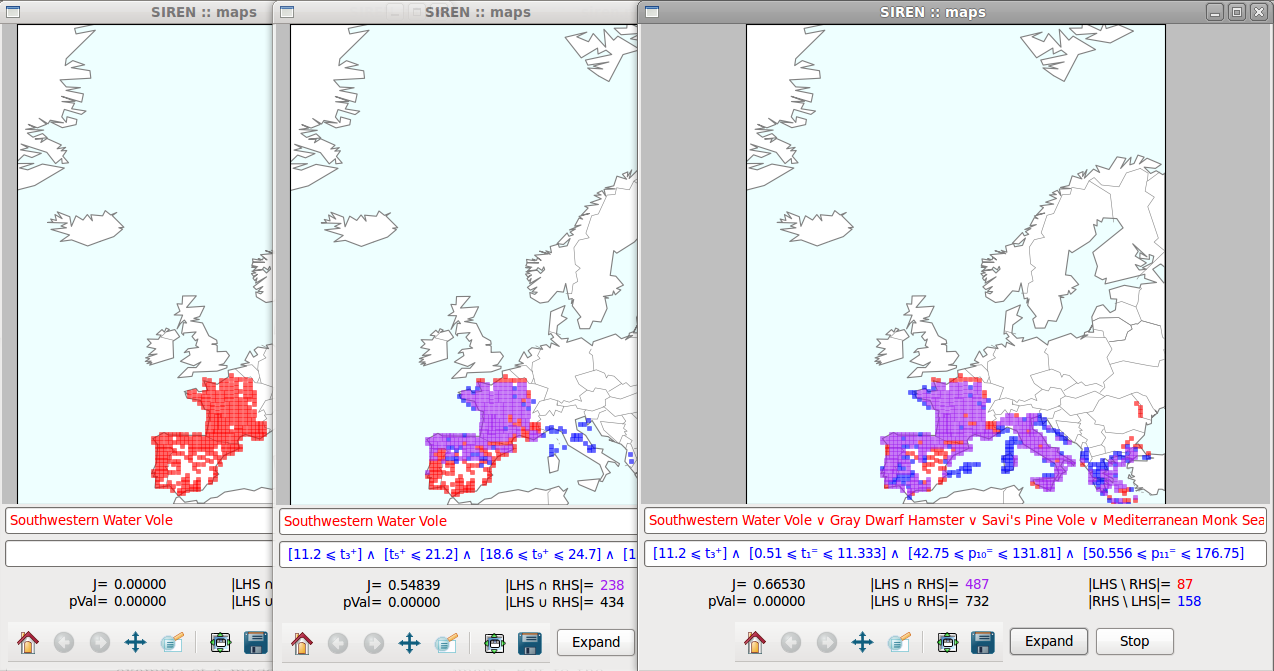
\includegraphics[width=0.7\textwidth]{screenshots/comparison}
  \caption{Several map panels. Comparing intermediate extensions automatically generated for a chosen starting variable. Red, blue and purple represents areas where only the left hand side query holds, only the right hand side query holds and where both queries hold, respectively.}
  \label{fig:comparison}
\end{figure}


\prg{Editing a redescription} It is typical that the user wants to
edit some of the obtained redescriptions. For example, some results
might be overly complex, or have exceedingly precise boundaries for
numerical variables. The user can easily select a redescription to
modify, open it in a map panel and edit it. Boundaries can be altered,
literals added or removed. \Siren\ \emph{instantly updates} the map and important
statistics (accuracy, $p$-value, etc.) of the redescription, allowing
the user to see the effects of the modifications immediately and
verify, e.g.\ whether the new redescription would still be acceptably
accurate.

Continuing with our example above, we might want to reduce the
precision of the climatic constraints to integers. We could edit the
query as follows:
\begin{equation*}
%\footnotesize
\begin{array}{l}
[11 \leq t_{3}^{+}] \land  [0 \leq t_{1}^{=} \leq 12]%\\[1mm]
%\quad
\land  [42 \leq p_{10}^{=} \leq 132] \land [50 \leq p_{11}^{=} \leq 177],
\end{array}
\end{equation*}
and obtain a redescription of slightly decreased accuracy. % of $0.659$.

\prg{Using subsets of variables} 
\Siren\ allows the user to specify variables to temporarily 
avoid when extending or mining redescriptions.
In our running example, we might want to force the
algorithm to search alternative redescriptions that do not involve any
 precipitation. For that purpose, we simply unselect all such
variables before running the extension anew. We will obtain the best
extensions containing only temperatures in the bioclimatic query, such
as the following redescription of accuracy $0.653$:
\begin{equation*}
%\footnotesize
\begin{array}{l}
\text{Southwestern Water Vole }\lor\text{ Cape Hare }\lor\text{ Savi's Pine Vole }\\[1mm]
\quad\lor\text{ Mediterranean Monk Seal}\\[3mm]
( [11.2 \leq t_{3}^{+}] \land  [20.1 \leq t_{7}^{+} \leq 32.9] %\\[1mm] 
%\quad 
\land  [0.51 \leq t_{1}^{=} \leq 11.333]) \lor  [34.0 \leq t_{8}^{+}].
\end{array}
\end{equation*}

Note that this redescription was not returned previously since the
beam search focused on better ones involving precipitation variables.
This feature allows the user to specify additional constraints,
thereby \emph{tuning the mining process} according to his interest and
what appears most promising during the analysis.

\prg{Filtering redundant redescriptions}
\label{sec:filt-redund-redescr}
The results returned during the extension
mentioned previously may contain many redundant redescriptions found
at different steps. We can easily sort them, e.g.\ by accuracy, select
one of interest and filter all the following results redundant with respect to it.

\prg{Sharing the results}
\label{sec:sharing-results}
Finally, \Siren\ facilitates \emph{distributing} the results:
redescriptions can be exported in easy-to-read format and the
maps associated to redescriptions can be readily converted to
publication-ready graphics. 

%%% Local Variables: 
%%% mode: latex
%%% TeX-master: "siren_iid"
%%% End: 

\section{Discussion}
\note{Use this section to open discussion (no conclusion section) ?}

This paper presents a tool for interactive and visual redescription
mining. While we believe that the goals---and the methods we present
to achieve them---are easy to accept as reasonable, we want to point
out that there are still many open problems, both conceptual and
technical, that need to be solved. 

In the heart of interactive data mining is the user's ability to tell
the algorithm that he wants more or less certain type of results. In
principle, this is no problem in \Siren: the user simply selects a
redescription he wants to remove from the beam search or extend
more. The problem, however, is that there can be (and usually are)
other, similar redescriptions that the user might also want to remove
or extend. He can do that manually, of course, but with larger number
of redescriptions, the process becomes very tedious very soon.

A solution to this problem would be to remove (or extend) all similar
redescriptions. But how to define the similarity? To give an example,
consider a case when the user finds a redescription saying that the
area where the Polar Bear lives is the area with January's mean
temperature below $-20$ degrees Celsius, in other words, Polar Bear
lives in cold. This is hardly a surprising result, and the user might
want to remove it (and other similar results) from the search. But we
can characterize the cold areas using other variables than just
January's mean temperature, so it is not enough to just stop extending
any redescription with Polar Bear and January's mean temperature in
it. Also, we cannot just remove all the redescriptions with Polar
Bear---that could remove some very interesting redescriptions,
too. Finally, we could consider the area in which the redescription
holds. But even that leaves a lot to be hoped for: if we remove all
redescriptions that contain that area, we probably remove too many
redescriptions, but if we restrict ourselves to the redescriptions
that are contained in the area, we probably miss most of the
redescriptions we should remove.  

The problem of removing and extending similar redescriptions is
closely related to that of redundancy reduction. There are often
multiple redescriptions that represent the same phenomenon (think of
the Polar Bears living in the cold areas), and ideally, we would like
to present the user only one of them. In other words, we do not want
to present the user any redescriptions that do not add any (or add
only marginally) new information over the redescriptions he has
already seen. But as with deciding which redescription is similar to a
selected one, also quantifying the redundancy between redescriptions
is a difficult problem.

% Data mining is an iterative process of refining hypotheses. The tool
% generates hypotheses about the data, here in the form of
% redescriptions. Then the user is able to select one, edit it, let the
% tool expand it. When satisfied with it, the user can remove redundant
% hypotheses and move on to the next one of interest. That is, at some
% point he is able to state that now, the information provided by the
% current hypothesis is admitted to be known, i.e. included in the
% knowledge and further hypotheses that does not add any information to
% that knowledge should be discarded.
% However, quantifying redundancy between hypothesis is a difficult problem.

% A data mining process is typically sparked by a question. But the
% question typically remains implicit and the analyist only formulates
% an hypothesis to answer it. Then, the mining tool can indicates
% whether the data supports the hypothesis, in other words help look for
% evidence supporting it. However, the fact that the hypothesis holds
% does not mean that it is the best answer to the original question.  In
% redescription mining, when considering an edited redescription (and
% mabye also in any case), the tool should allow to evaluate the
% significance and interestingness of the redescription using \pValue{}s
% or randomization techniques.  Other related results, redescriptions
% covering roughly the same area, containing the same variables or
% having similar statistics, should be suggested to provide context to
% the current redescription and challenge that hypothesis.

When interpreting a redescription, one should always bear in mind
the assumptions attached to it. For example, whether some variables
were disabled or whether the focus was put on some area when it was
generated.  Hence, keeping track of the constraints used when mining a
redescription is essential. However, if the user is allowed to stop
the extension process, modify the constraints and resume the search,
this might be fairly intricate and interpretation of the results
become impossible.

The goal of data mining is to find new and interesting information
from the data. In interactive data mining in general, and with the
tools discussed in this paper in particular, the user can guide the
data mining method towards the results he prefers. This raises new
problems. First, we have to control that the data supports the results
the user finds and second, we must be careful that the user actually
finds new information, not just the information he already knew. 

The first problem, making sure that the obtained results are supported
by the data, is ages old in sciences. In short, it is the question of
testing the significance of a hypothesis, and there is a vast body of
statistical literature about it. Our proposed algorithms mitigate the
problem by computing a $p$-value, but as it is based on a fixed null
hypothesis, it is not adequate in every case.

The second problem is more conceptual: taken to an extreme, the
interactivity removes the data mining from the interactive data
mining. If the user more or less directly tells the algorithm the
redescription he wants to see, the \Siren\ program turns into a mere
plotting interface. Even on the less extreme case, the user can easily
(an unwittingly) guide the algorithm towards the kind of results he
wanted to see. Together with the fact that we can only check against a
fixed null hypothesis, this causes a considerable risk of false
findings. The onus is on the user to make sure he does not misuse the algorithm.

% It is possible to evaluate a completely hand-crafted redescription. Is this a problem? Why?
% What is the difference between generating hypotheses from the data versus backing hypotheses with the data.
% How to avoid that the user finds what he is looking for and only that?
% That is, a tool not to explore data and formulate new hypotheses, but to find arguments to support pre-existing theories?

%%% Local Variables: 
%%% mode: latex
%%% TeX-master: "siren_iid"
%%% End: 


%\bibliographystyle{abbrv}
\bibliographystyle{splncs03}
%\nocite{*}
\bibliography{bibsiren}  
\end{document}

%%% Local Variables: 
%%% mode: latex
%%% TeX-master: t
%%% End: 



% \begin{figure}[hb]
%   \centering
% 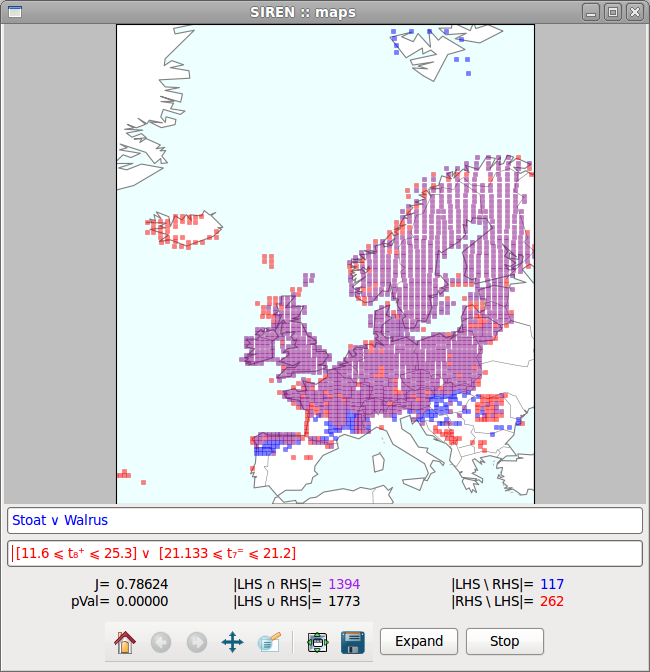
\includegraphics[width=.5\textwidth]{screenshots/siren_map.png}
%   \caption{Map panel, displaying a redescription on a map.}
%   \label{fig:map_panel}
% \end{figure}


% \begin{figure}
%   \centering
% 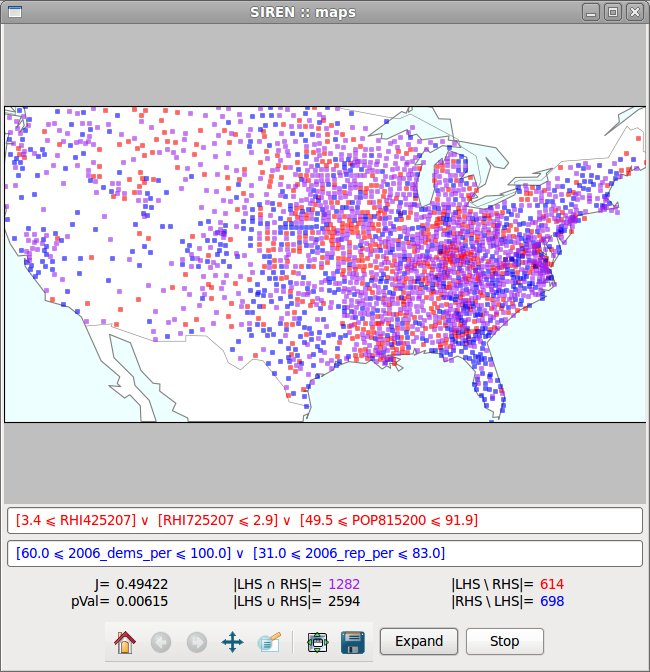
\includegraphics[width=.5\textwidth]{screenshots/siren_map_us_00.jpg}
%   \caption{Map panel, displaying a redescription on a map.}
%   \label{fig:map_panel}
% \end{figure}

% \begin{figure}
%   \centering
% 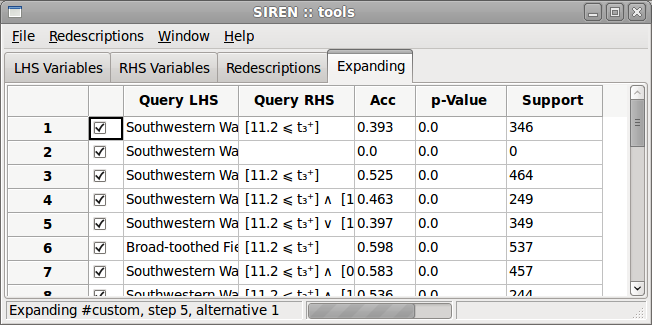
\includegraphics[width=0.5\textwidth]{screenshots/extending.png}
%   \caption{Tool panel. Intermediates results found during the extension of a redescription.}
%   \label{fig:extending}
% \end{figure}

% \begin{figure}
%   \centering
% 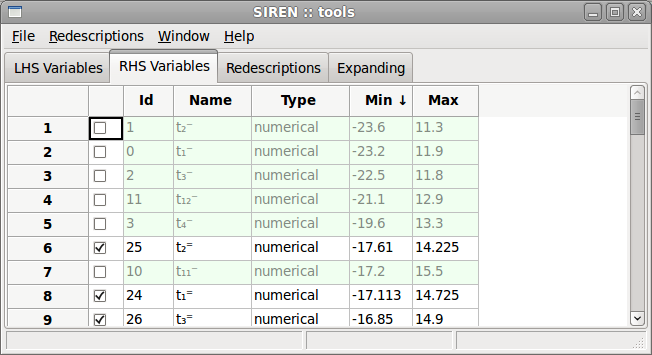
\includegraphics[width=.5\textwidth]{screenshots/variables_05.png}
%   \caption{Tool panel, uselecting variables.}
%   \label{fig:map_panel}
% \end{figure}

% \begin{figure}
%   \centering
% 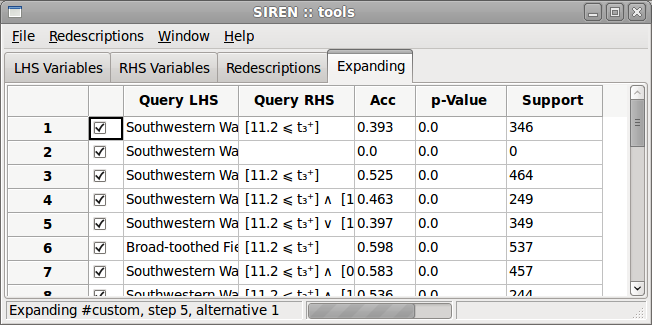
\includegraphics[width=0.5\textwidth]{screenshots/extending.png}
%   \caption{Tool panel, extending a redescription.}
%   \label{fig:extending}
% \end{figure}

% \begin{figure}
%   \centering
% 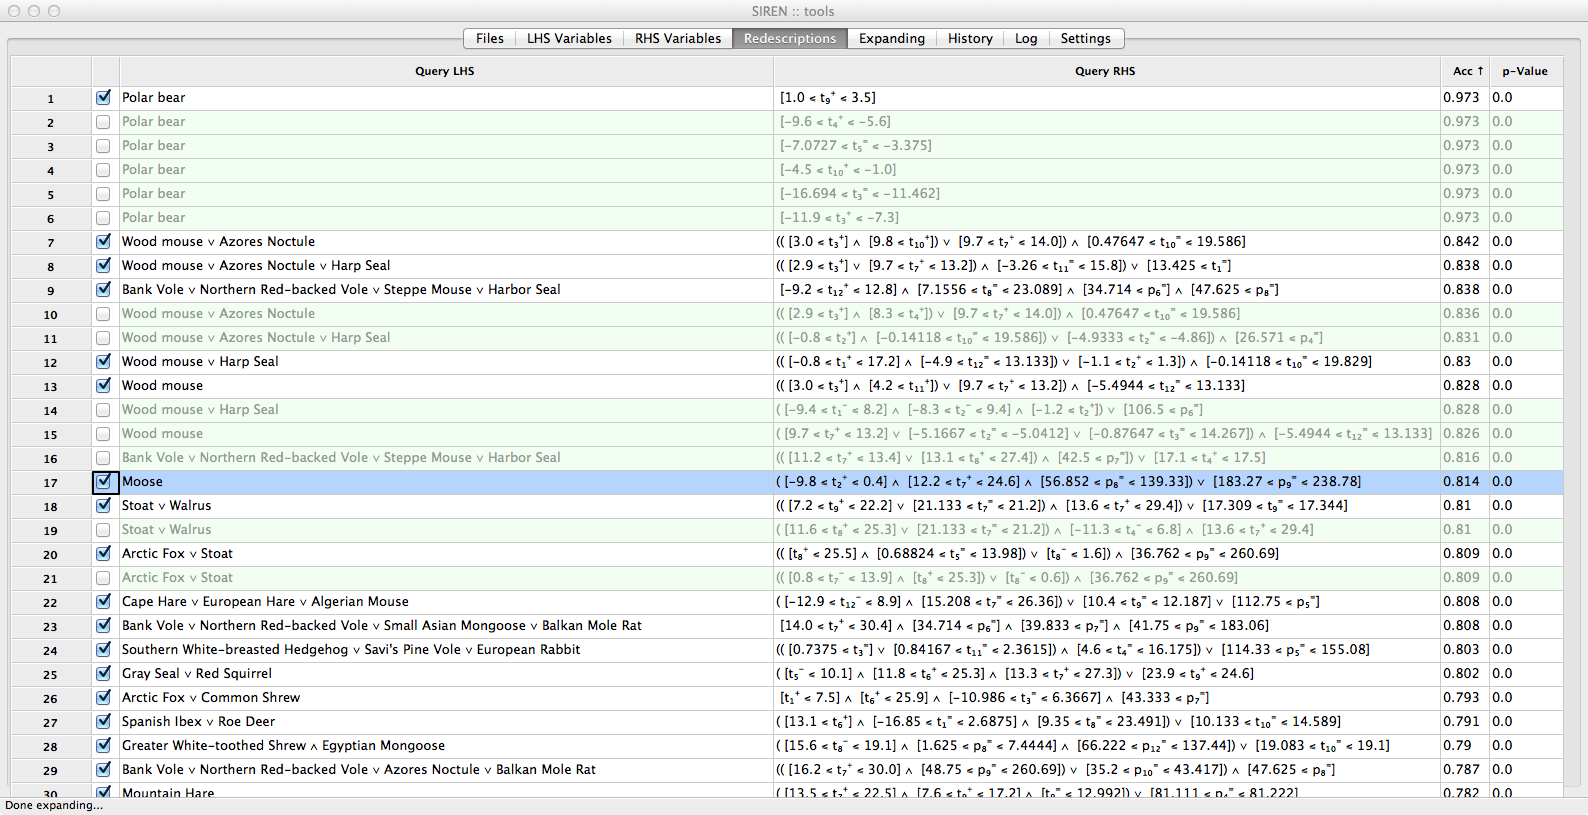
\includegraphics[width=.5\textwidth]{screenshots/redescriptions.png}
%   \caption{Tool panel, filtering redescriptions.}
%   \label{fig:filtering}
% \end{figure}

% LocalWords:  throught siid screenshots uselecting
